\documentclass[../main.tex]{subfiles}
\graphicspath{{\subfix{../figures/}}}

\begin{document}
\chapter{Introduction} \label{chap:intro}


\section{Report Organization}
This thesis is divided into six primary chapters. First, this introductory chapter provides an overview of the application, explains the rationale behind the research, and outlines the tasks involved. The next one, chapter \ref{chap:baseline}, presents the current facility and achievement at OJ Electronics A/S as a standard benchmark. Chapter \ref{chap:review} follows with a thorough examination of related literature around the world to identify the most suitable approach. Then, chapter \ref{chap:ctrl_design} delves into the detailed execution of the project, discussing the design and various techniques employed to achieve optimal performance. Several issues that arise during the hardware integration phase are resolved in chapter \ref{chap:hw}. Finally, chapter \ref{chap:eval} reveals the test results of our proposal and its performance in various scenarios and compares it with the existing UWG5 PI controller before concluding the whole thesis.

Additionally, the initial sections alongside the Table of Contents from page i to xii provide more details about figures, data tables, acronyms, and mathematical notation. Appendix \ref{chap:apa} provides MATLAB/Simulink source code for later reproduction. These supplementary pages are to enhance readers' understanding and provide comprehensive insights into the research.


\section{Application Background}
Room heating is a fundamental function of a high-quality living space. Its primary purpose is to maintain a comfortable temperature for the occupants. Whether on a cool autumn day or a chilly winter night, heating ensures we can live and work comfortably indoors. Properly heated rooms also contribute to our overall health, preventing cold-related illnesses while enhancing productivity. Effective heating solutions can also protect the home itself, preventing issues such as frozen pipes and condensation, which can lead to structural damage over time. In essence, a reliable heating system is crucial for both comfort and safety in our living environments.
\begin{figure}[H]
    \centering
    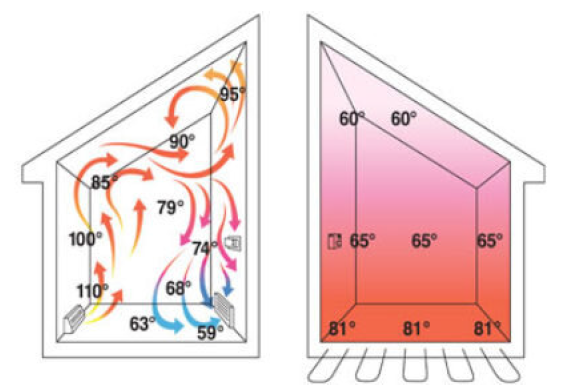
\includegraphics[width=0.8\linewidth]{figures/room_heating_setups.png}
    \caption{Forced air heating (FAH) vs. floor heating (FHE)\cite{junior22}}
    \label{fig:room_heating_setups}
\end{figure}

A popular method for temperature regulation is the use of a forced air heating (FAH) system, thanks to its quick response and relatively cheap installation. FAH systems work by drawing air into a furnace, where it is heated and then distributed throughout the building via a network of ducts. Despite its efficiency, FAH systems have several drawbacks. They cannot distribute heat evenly due to their turbulent air movement, which often results in hot and cold spots within a room. Figure \ref{fig:room_heating_setups} even shows that FAH equipment can be bulky and occupy valuable space within the home.

An alternative for distributing heat more evenly is the use of an underfloor heating (FHE) system, which warms the room from the ground up. These methods involve installing heating elements or water-filled pipes beneath the floor, providing a consistent and gentle heat that radiates upward. They offer several advantages over FAH systems. They ensure more uniform heat distribution, are completely hidden from view, and do not take up any space within the living area. The lack of moving air also reduces the circulation of dust and allergens, contributing to a healthier indoor environment.

There are two main types of FHE technologies: electric and hydronic. Electric systems use electrical resistance cables or mats to generate heat. They are typically easier and less expensive to install, making them a popular choice for retrofitting existing buildings or heating small areas such as bathrooms and kitchens. Hydronic systems, on the other hand, circulate warm water through a network of pipes embedded in the floor. They are more complex and usually more costly to install than electric ones, but they are more efficient and economical to run, especially in larger areas. Hydronic systems often exist in new construction or major renovations, where long-term energy savings can offset the initial installation costs.

In both technologies, a thermostat regulates the temperature by controlling the flow of electricity or water through the heating elements. Advanced thermostats often use proportional-integral (PI) controllers to modulate the heat output precisely. When the room temperature falls below the desired setpoint, the thermostat increases the current through the electric coils or the flow of warm water through the pipes, generating more thermal energy to heat the room. As the room temperature approaches the setpoint, it reduces the current or water flow, maintaining a stable and comfortable indoor climate.

\nomenclature[D]{FAH}{Forced Air Heating, a room heating technology}
\nomenclature[D]{FHE}{Floor Heating, a better alternative to FAH. There are two main technologies: electrical and hydronic.}
\nomenclature[D]{PID}{Proportional-Integral-Derivative, the most common controller used in various industries}
\nomenclature[D]{PI}{Proportional-Integral, a variation of PID without the derivative term}


\section{Motivation for Improvement}
OJ Electronics A/S (OJ) is the Danish market leader in electric floor heating systems (FHE). Having been in business for more than 60 years, we realize that conventional FHE designs are not adaptive to the rapid change of Northern European weather. However, they consume a lot of energy. Nonetheless, they can only operate on a fixed schedule, making it hard to personalize and fulfill modern users' needs. Finally, floor heating contexts are always difficult to present correctly in mathematics, making them inappropriate for model-based optimal control schemes.
\begin{figure}[H]
    \centering
    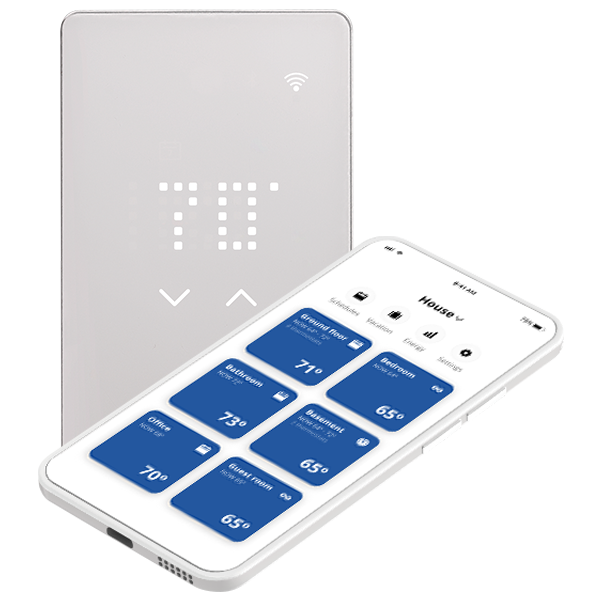
\includegraphics[width=0.6\linewidth]{figures/uwg5.png}
    \caption{UWG5 thermostat from OJ Electronics}
    \label{fig:uwg5}
\end{figure}

On the other hand, artificial intelligence (AI) is emerging in various control systems. They leverage measured data to yield better decisions without relying on complex mathematical models, effectively mimicking human learning processes. Just as humans learn from their mistakes to make improved decisions, AI systems enhance their performance through iterative data analysis. Thus, we aim to advance our product research and development forward in this direction and have the first AI-enabled prototype released soon. The target hardware is UWG5, our latest thermostat. This device has all the bells and whistles for a modern smart home, e.g., a pocket-size form factor, Amazon Alexa integrated, remote control via Google Home, etc.

\nomenclature[D]{OJ}{OJ Electronics A/S, the Danish corporation that supports this thesis.}

\section{Problem Statement}
Many prior articles, including two student theses at OJ that used Deep Q-Network (DQN) and Advantage Actor-Critic (A2C), demonstrate impressive floor heating control performance. Yet, most of them rely on unrealistic software simulations, either with Energy Plus or SimScape. By thoroughly investigating an actual plant in various scenarios, this thesis aims to prove if their claims are feasible. In other words, we seek the answers to two key questions: "When can reinforcement learning (RL) outperform a traditional controller?" and "Can an undiscovered RL solution be even better?" The outcome would contribute more practical insights into energy-efficient alternatives for the HVAC industry and household energy management systems.

\nomenclature[D]{DQN}{Deep Q-Network, an RL agent of discrete action}
\nomenclature[D]{A2C}{Advantage Actor-Critic, an RL agent of continuous action, based on the Actor-Critic framework}


\section{Scope of Work}
According to the problem statement, this thesis encompasses several tasks. First, we construct a mathematical model of the real environment using thermodynamics and physical data recorded at OJ. This model serves as a foundation for training and evaluating the studied algorithm. Next, we establish a performance baseline for the UWG5's Proportional-Integral (PI) controller. Subsequently, we proceed to train, assess, and flash the model into a microcontroller as a standalone function. Finally, we benchmark their on-chip performance against a common set of predefined criteria.

In contrast, it is essential to delineate the tasks that fall outside the above list. First, we do not have the purview of integrating our AI model with a fully functional UWG5 thermostat. Also, quantifying "user comfort" based on individual preferences and exploring model-based techniques (e.g., Model Predictive Control or Linear Quadratic Regulator) are off the table.

\end{document}